\documentclass[french,a4paper]{scrartcl}
\input{eval.latex}
%%%%%%%%%%%%%%%%
\def\Classe{TSTMG}
\def\Titre{Évaluation : Variable aléatoire / Loi binomiale}
\def\NoterSur{25}
%%%%%%%%%%%%%%%%
\begin{document}
\DoTitle
\exo{Chapitre précédent - Statistiques \exosur{5}}{
	On \faDiceOne~s'intéresse à l'évolution de la fréquentation des camping 4 étoiles ou plus en France métropolitaine.
	\vspace*{2mm}
	\begin{center}
		\def\arraystretch{1.2}
		\begin{tabular}{|l|c|c|c|c|c|c|c|}\hline
			Année                                        & 2004   & 2005   & 2006   & 2007   & 2008   & 2009   & 2010   \\ \hline
			Rang de l'année : $x_i$                      & 0      & 1      & 2      & 3      & 4      & 5      & 6      \\ \hline
			Fréquentation en milliers de nuitées : $y_i$ & 25 156 & 26 470 & 28 295 & 28 897 & 30 063 & 31 212 & 32 014 \\ \hline
		\end{tabular}
	\end{center}
	\vspace*{2mm}
	Le nuage de points de coordonnées $(x_i ; y_i)$ pour $i$ variant de $0$ à $6$ est représenté en  annexe.
	\vspace*{2mm}
	\begin{enumerate}
		\q{1} Déterminer le taux d'évolution du nombre de nuité entre 2004 et 2010.
		\q{1} À l'aide de la calculatrice, déterminer une équation de la droite d'ajustement affine de $y$ en $x$ obtenue par la méthode des moindres carrés (arrondir les coefficients au \textbf{dixième}).
		\item On décide d'ajuster le nuage avec la droite $(D)$ d'équation $y = 1~150x+25~500$.
		      \begin{enumerate}
			      \q{1} Tracer la droite $(D)$ sur le graphique de l'annexe.
			      \q{1} Déterminer graphiquement le nombre de nuitées prévu par ce modèle en 2014. Faire apparaître les tracés utiles.
			      \q{1} Déterminer à partir de quelle année le nombre de nuitées prévu par ce modèle sera supérieur à $48~000$.
		      \end{enumerate}
	\end{enumerate}
}

\newpage~\newpage

\exo{Téléphones et espérance \exosur{4}}{
	\img{2cm}{img/tel}
	Une entreprise produit des écrans pour téléphones portables. Ces écrans peuvent présenter 2 défauts : un défaut de dimension ou un défaut de résistance au choc.

	La probabilité qu'un écran pris au hasard présente uniquement un défaut est de $0,07$ et la probabilité qu'il présente deux défauts et de $0,04$.

	Soit $X$ la variable aléatoire qui, a tout écran de cette production pris au hasard, associe le nombre de défauts.
	\begin{enumerate}
		\q{1} Quelles sont les valeurs prises par $X$ ?
		\q{2} Donner sous forme de tableau la loi de probabilité de $X$.
		\q{1} Déterminer l'espérance de $X$.
	\end{enumerate}
}
\newpage
\exo{Pile ou Face truqué \exosur{4}}{
	\img{2.5cm}{img/piece}
	On lance $3$ fois une pièce de monnaie truquée telle que la probabilité d'obtenir PILE est $0,42$. Soit $X$ la variable aléatoire comptant le nombre de PILE obtenus.
	\begin{enumerate}
		\q{1} Justifier que $X$ suit la loi binomiale dont vous préciserez les paramètres.
		\q{2} Représenter cette situation par un arbre pondéré
		\q{1} Calculer et interpréter $P(X = 1)$
	\end{enumerate}
}
\newpage
\exo{Stylos \exosur{4}}{
	\img{1.9cm}{img/stylo}
	Une usine fabrique en grande quantité un certain modèle de stylo.

	On prélève un stylo au hasard dans une importante livraison destinée à une chaîne d'hypermarchés.

	On note $D$ l'événement : "un stylo prélevé au hasard est défectueux" et on suppose que $P(D) = 0,016$.

	À la rentrée scolaire ce type de stylo est vendu par lot de $6$ dans ces hypermarchés.

	On prélève au hasard $6$ stylos dans la livraison pour vérification.

	On considère la variable aléatoire $X$ qui, à tout prélèvement de $6$ stylos, associe le nombre de stylos défectueux de ce prélèvement.

	\begin{enumerate}
		\q{1} Justifier que là variable $X$ suit une loi binomiale dont on déterminera les paramètres
		\q{1} Calculer la probabilité que, dans un tel prélèvement, il y ait aucun stylo défectueux.
		\q{1} En déduire la probabilité que, dans un tel prélèvement, il y ait \textbf{au moins} un stylo défectueux.
	\end{enumerate}
}
\newpage

\exo{Angine et loi de probabilité \exosur{8}}{
	\ul{\textbf{Partie A}}
	\img{2cm}{img/angine}
	L'angine chez l'être humain est provoquée soit par une bactérie soit par un virus. On admet qu'un malade ne peut pas être à la fois porteur du virus et de la bactérie et l'angine est bactérienne dans 20\% des cas.

	Pour déterminer si une angine des bactériennes on dispose d'un test dont le résultat peut être positif ou négatif.

	Le test est conçu pour être positif lorsque l'angine est bactérienne mais il présente des risques d'erreur :

	\begin{itemize}
		\item Si l'angine est bactérienne, le test est négatif dans 30\% des cas.
		\item Si l'angine est virale le test est positif dans 10\% des cas.
	\end{itemize}

	On note les événements :
	\begin{itemize}
		\item $B$ : "l'angine est bactérienne"
		\item $T$ : "le test est positif"
	\end{itemize}

	On rappelle que si $E$ et $F$ sont 2 événements, $P(E)$ désigne la probabilité de $E$ et $P_{F}(E)$ désigne la probabilité de $E$ sachant que $F$ est réalisé. On note $\overline{E}$ l'événement contraire de $E$.

	\begin{enumerate}
		\q{1} Représenter la situation par un arbre de probabilité
		\q{1} Quelle est la probabilité que l'angine du malade soit bactérienne \textbf{et} que le test soit positif ?
		\q{1} Montrer que la probabilité que le test soit positif est de 0,22.
		\q{1} \textbf{Sachant qu}'un malade est testé est positif, quelle est la probabilité que son angine soit bactérienne ?
	\end{enumerate}

	\ul{\textbf{Partie B}}

	On choisit au hasard $5$ malades atteints d'une angine. On note $X$ la variable aléatoire qui donne, parmi les $5$ malades choisis, le nombre de malades dont le test est positif.

	\begin{enumerate}[resume]
		\q{1} Quelle est la loi de probabilité suivie par $X$. Préciser ces paramètres.
		\q{1} Calculer et interpréter $P(X = 2)$
		\q{1} Calculer la probabilité qu'au moins l'un des $5$ malades est un test positif.
		\q{1} Calculer et interpréter l'espérance mathématique de $X$.
	\end{enumerate}

}
\newpage~\newpage\backgroundsetup{contents={}}
~\\~
\begin{center}
	\textbf{\LARGE{Annexe - Exercice n°1}}
\end{center}
~\\~
\begin{center}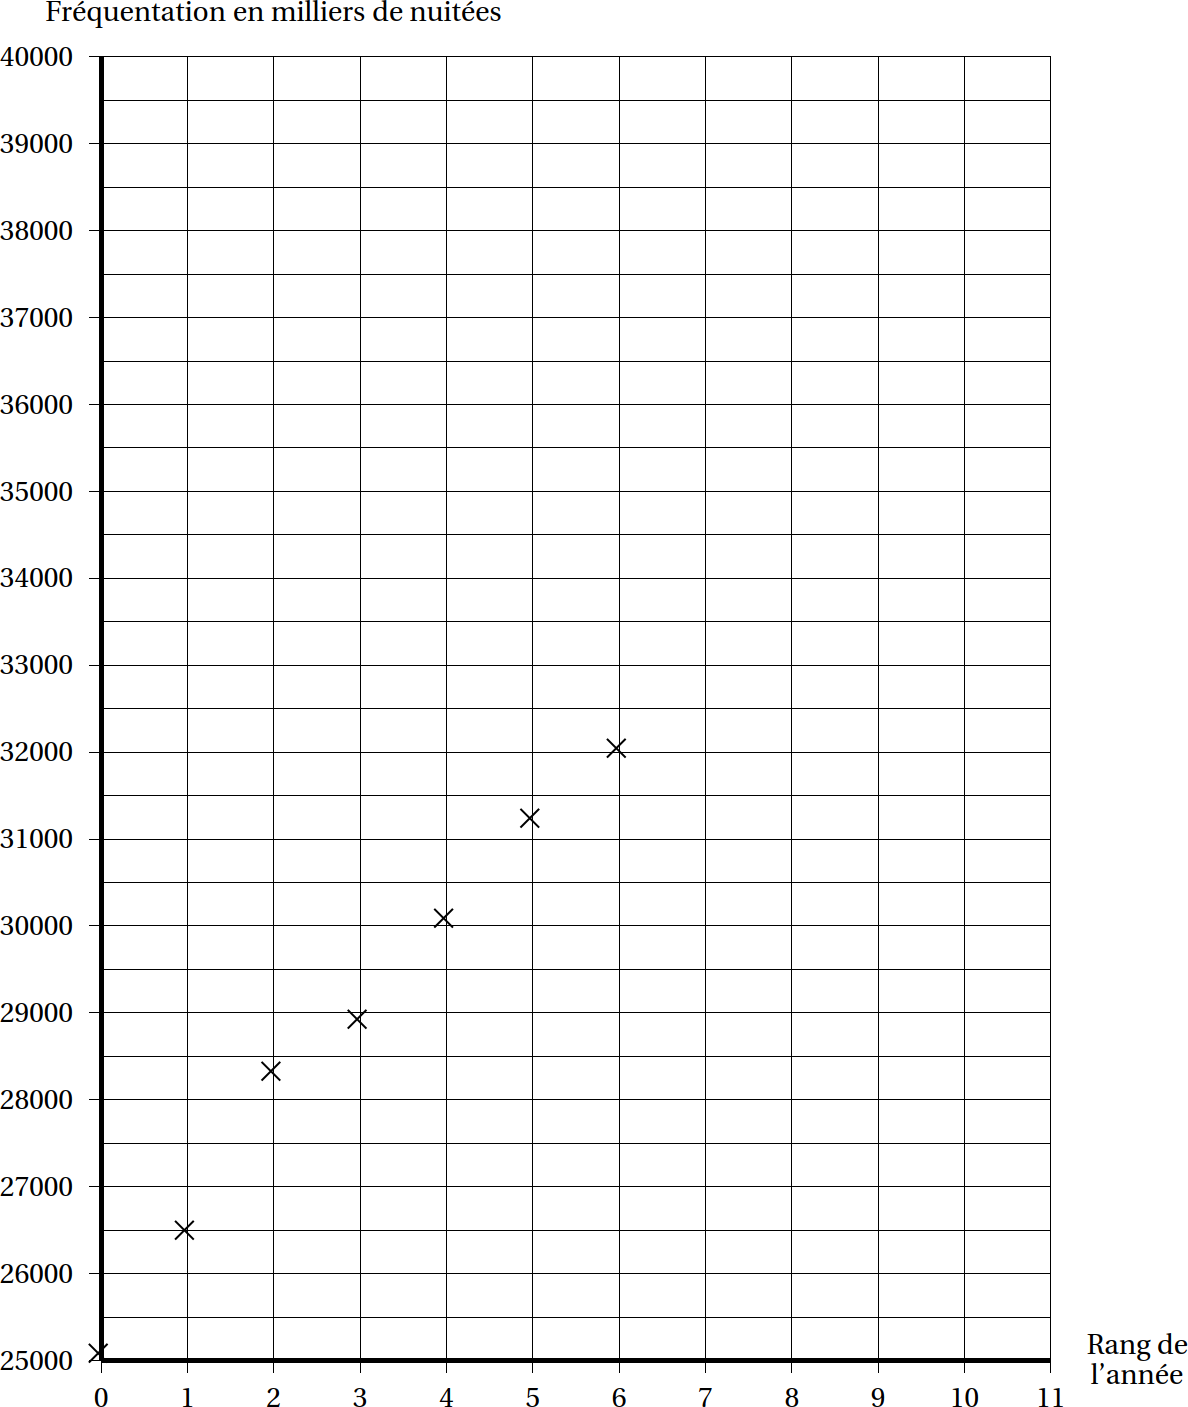
\includegraphics[width=18.5cm]{img/annexe}\end{center}
\end{document}
